\chapter{Программная реализация анализатора и инфраструктуры}

Данная реализация анализатора является первичной и её главная задача это иллюстрация работоспособности метода анализа.
Поэтому данный анализатор включает дополнительную инфраструктуру, не рассматриваемую в методе. Такие компоненты
анализатора будут отмечены соответствующим примечанием в тексте.

\section{Общая архитектура}

\subsection{Составляющие анализатора}

Исходя из раздела \ref{sec:architecture} анализатор, реализующий описываемый метод мультиязыкового анализа будет включать в себя следующие
компоненты:
\begin{enumerate}[1)]
    \item провайдер конфигурации и кода,
    \item мультиязыковой транслятор,
    \item решатель ограничений,
    \item адаптер для конкретного инструментального средства (в данном случае LSP сервера).
\end{enumerate}

Более подробный состав анализатора представлен на диаграмме компонентов на рисунке \ref{fig:components}.

\begin{figure}[H]
    \centering
    \resizebox{0.9\linewidth}{!}{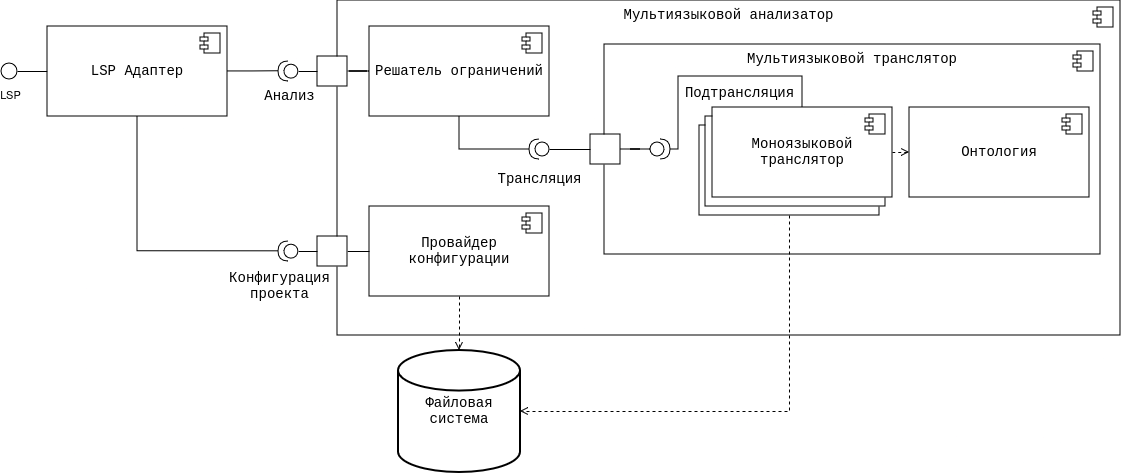
\includegraphics[height=0.85\textheight]{inc/img/components}}
    \caption{Диаграмма компонентов анализатора}
    \label{fig:components}
\end{figure}

Также, порядок запросов к анализатору и вызовы соответствующих процедур приведены на диаграмме деятельности
на рисунке \ref{fig:sequence}.

\begin{figure}[H]
    \centering
    \resizebox{\linewidth}{!}{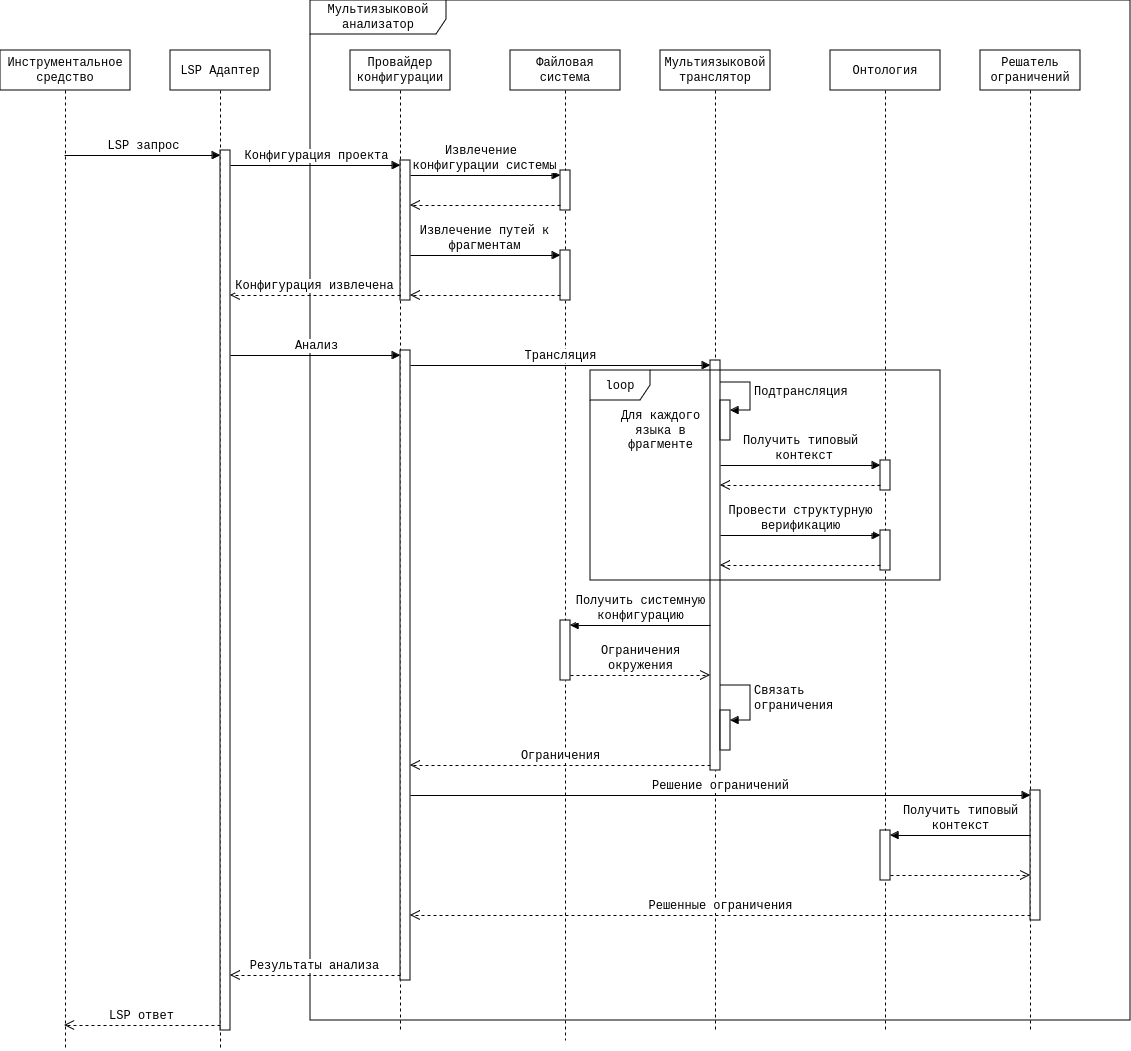
\includegraphics[height=0.85\textheight]{inc/img/sequence}}
    \caption{Диаграмма деятельности анализатора}
    \label{fig:sequence}
\end{figure}

Стоит сразу уточнить несколько деталей относительно представленных диаграмм:
\begin{enumerate}[1)]
    \item диаграммы представлены на русском языке, на довольно высоком уровне -- это сделано с целью упрощения
    понимания компонентов анализатора,
    \item на диаграммах не представленно кеширование результатов анализа на различных этапах,
    \item на диаграмме деятельности представлен самый благоприятный сценарий, без возникновения ошибок -- в случае ошибок
    используется стандартный механизм возврата ошибок JSON-RPC \cite{JSON-RPC}.
\end{enumerate}

\subsection{Протоколы взаимодействия}

Приведенные на рисунке \ref{fig:components} интерфейсы компонентов являются протоколами взаимодействия.
Каждый компонент в сущности представляет собой отдельное приложение, поэтому такие протоколы описывают в первую очередь межпроцессное взаимодействие.
Такой подход к структуре анализатора был сделан по следующим причинам:
\begin{enumerate}[1)]
    \item увеличение гибкости анализатора для расширения (в первую очередь в части количества моноязыковых трансляторов),
    \item поддержка использования многозадачности системы для одновременного анализа множества фрагментов,
    \item поддержка различных языков и технологий реализации компонентов.
\end{enumerate}

Стоит обратить внимание на заключительный пункт -- в отличие от некоторых мультиязыковых анализаторов, рассмотренных в разделе \ref{sec:num2},
подход с использованием обобщенной модели и общего протокола позволяет абстрагироваться от деталей реализации конкретного транслятора.
Это может быть полезно к примеру в том случае, если для анализируемого языка уже существует инфраструктура для анализа и она на другом языке
(чаще всего на нем самом). 

К примеру, можно привести инфраструктуру LLVM и в частности Clang для анализа C++ --
в проекте существует множество различных инструментов анализа C++, от построения AST и CFG до проведения различных оптимизаций.
Разработчик моноязыкового транслятора может использовать эту инфраструктуру свободно, в его обязанность входит лишь
сопровождение результатов анализа в опредленной протоколом форме.
Этот факт, в свою очередь, в целом позволяет использовать различные техники статического анализа (межпроцедурный анализ, построение DFG,
абстрактная интерпретация) что повышает гибкость моноязыковых трансляторов без изменения всего анализатора. 

Каждый из используемых протоколов базируется на механизме JSON-RPC. Это позволяет учесть стандартные
сценарии возникновения ошибок при передаче данных или во время анализа, а также устанавливает
совместимость с популярными инструментами (в первую очередь LSP). Описание протоколов
приведено в приложении \ref{cha:appendix1}. В качестве языка описания используется TypeScript так как
его типовые определения имеют достаточно высокую выразительность и его типы напрямую могут быть отражены в типы JSON.

\subsection{Реализация онтологии}

Как сказано в подразделе \ref{ssec:ontology}, онтология в данной работе является собирательным названием
механизмов поддержания консистентности.

Программная реализация таких механизмов была сделана при помощи использования отдельной виртуальной машины
в мультиязыковом трансляторе \cite{goja}. Такая машина является встраиваемым в приложение решением и
направлена на исполнение кода JavaScript.

Подход по встраиванию виртуальной машины был избран по следующим причинам:
\begin{itemize}
    \item скрипты JavaScript являются отдельной точкой расширения мультиязыкового анализатора и не затрагивают его компоненты, что повышает
    модульность,
    \item JavaScript является самым удобным средством для работы с JSON, так как является его суперсетом,
    \item использование полноценного языка программирования в отличие от языка описания данных позволяет
    без излишнего усложнения расширять функциональность онтологии.
\end{itemize}

\section{Провайдер конфигурации и кода}

\section{Мультиязыковой транслятор}

\section{Решатель ограничений}

\section{Адаптер инструментального средства}

% TODO: Протокол анализатора
% TODO: Кэш компонентов